%
% auth: Mattijs Korpershoek
% mail: <mattijs.korpershoek@gmail.com>
%
\documentclass[compress]{beamer}
%%%%%%%%%%%%%%
%  Packages  %
%%%%%%%%%%%%%%
\usepackage[english]{babel}
\usepackage[T1]{fontenc}
\usepackage{lmodern}
\usepackage{microtype}
\usepackage{multicol}
\usepackage[normalem]{ulem}
\usepackage{soul}
\usepackage{listings}
\usepackage{caption}
\usepackage{textpos} % for textblock
\usepackage{mathtools} % math environment
\usepackage{textcomp}
\usepackage{pgfgantt}
\usepackage{dirtree}

%%%%%%%%%%%%%%%%%%%%%
% Special variables %
%%%%%%%%%%%%%%%%%%%%%
\newcommand{\ImageFolder}{./img}

%%%%%%%%%%%%%%%%%%%%%%%
% Beamer environments %
%%%%%%%%%%%%%%%%%%%%%%%
% sets automatically the current subsection as frame title on your slide
\newenvironment<>{FrameWithSubSection}%
{%
  \begin{frame}%
    \frametitle{\insertsubsectionhead}%
    \par%
  }
  {%
    \par%
  \end{frame}%
}
% the % are at the end of each line because with some text editors,
% the LaTeX compiler may understand the \n as a command caracter.

%%%%%%%%%%%%%%%%%%%%%%
%  Solarized colors  %
%%%%%%%%%%%%%%%%%%%%%%
\definecolor{base03}{HTML}{002B36}
\definecolor{base02}{HTML}{073642}
\definecolor{base01}{HTML}{586E75}
\definecolor{base00}{HTML}{657B83}
\definecolor{base0}{HTML}{839496}
\definecolor{base1}{HTML}{93A1A1}
\definecolor{base2}{HTML}{EEE8D5}
\definecolor{base3}{HTML}{FDF6E3}
\definecolor{yellow}{HTML}{B58900}
\definecolor{orange}{HTML}{CB4B16}
\definecolor{red}{HTML}{DC322F}
\definecolor{magenta}{HTML}{D33682}
\definecolor{violet}{HTML}{6C71C4}
\definecolor{blue}{HTML}{268BD2}
\definecolor{cyan}{HTML}{2AA198}
\definecolor{green}{HTML}{859900}



%%%%%%%%%%%%%%%%%%%%
% caption settings %
%%%%%%%%%%%%%%%%%%%%
\DeclareCaptionFont{captionText}{\color{base1}}
\DeclareCaptionFormat{listing}{\colorbox{base03}{\parbox{0.985\textwidth}{\hspace{15pt}#1#2#3}}}
\captionsetup[lstlisting]{format=listing,labelfont=captionText,textfont=captionText, singlelinecheck=true, margin=0pt, font={sf,footnotesize}}
\DeclareCaptionFormat{figure}{\colorbox{base03}{\parbox{0.985\textwidth}{\hspace{15pt}#1#2#3}}}
\captionsetup[figure]{format=figure,labelfont=captionText,textfont=captionText, singlelinecheck=false, margin=0pt, font={sf,footnotesize}}

\lstdefinelanguage{pfwLang}
{morekeywords={Domain, Conf, Component},
sensitive=false,
morecomment=[l]{\#},
morestring=[b]",
}

\usepackage{inconsolata}
\lstset{
    basicstyle=\ttfamily\footnotesize,
    language=C,
    frame=lines,
    sensitive=true
    tabsize=2,
    breaklines=true,
    showstringspaces=false,
    showspaces=false,
    backgroundcolor=\color{base3},
    keywordstyle=\color{blue},
    commentstyle=\color{base1},
    stringstyle=\color{cyan},
    numberstyle=\color{violet},
    rulecolor=\color{base00},
    morekeywords={pfw, setParameter, getParameter}
}

\lstnewenvironment{code}[1][]%
{
    \noindent
    \minipage{\linewidth}
    \vspace{0.5\baselineskip}
        \lstset{#1}}
{\endminipage}

%%%%%%%%%
% fonts %
%%%%%%%%%
\usefonttheme[onlymath]{serif}
\usepackage{fontspec}
\defaultfontfeatures{Mapping=tex-text}
\setsansfont[Ligatures={Common}]{Futura}

%%%%%%%%%%%%%%%%
% Beamer Theme %
%%%%%%%%%%%%%%%%
%\usetheme{Warsaw}

\useinnertheme{circles}
\useoutertheme{split}

%\usecolortheme[RGB={255,51,0}]{structure} % Paul sabatier red logo color

%\setbeamercolor{alerted text}{fg=orange}
%\setbeamercolor{background canvas}{bg=base3}
%\setbeamercolor{block body alerted}{bg=normal text.bg!90!black}
%\setbeamercolor{block body example}{bg=normal text.bg!90!black}
%\setbeamercolor{block title alerted}{use={normal text,alerted text},fg=alerted text.fg!75!normal text.fg,bg=normal text.bg!75!black}
%\setbeamercolor{block title example}{use={normal text,example text},fg=example text.fg!75!normal text.fg,bg=normal text.bg!75!black}
%\setbeamercolor{fine separation line}{}
%\setbeamercolor{frametitle}{fg=base3}
%\setbeamercolor{item projected}{fg=black}
%\setbeamercolor{normal text}{bg=base2,fg=base02}
%\setbeamercolor{palette sidebar primary}{use=normal text,fg=normal text.fg}
%\setbeamercolor{palette sidebar quaternary}{use=structure,fg=structure.fg}
%\setbeamercolor{palette sidebar secondary}{use=structure,fg=structure.fg}
%\setbeamercolor{palette sidebar tertiary}{use=normal text,fg=normal text.fg}
%\setbeamercolor{section in sidebar}{fg=orange}
%\setbeamercolor{section in sidebar shaded}{fg=grey}
%\setbeamercolor{separation line}{}
\setbeamercolor{sidebar}{bg=blue}
\setbeamercolor{structure}{fg=blue}
%\setbeamercolor{subsection in sidebar}{fg=brown}
%\setbeamercolor{subsection in sidebar shaded}{fg=grey}
%\setbeamercolor{title}{fg=brown}
%\setbeamercolor{titlelike}{fg=brown}
\setbeamercolor{block body}{bg=base2 text.bg!90!base02}
\setbeamercolor{block title}{bg=blue}

\usetheme{Berlin}
\useoutertheme[]{miniframes}

\defbeamertemplate*{footline}{shadow theme}
{%
  \leavevmode%
  \hbox{\begin{beamercolorbox}[wd=.5\paperwidth,ht=2.5ex,dp=1.125ex,leftskip=.3cm plus1fil,rightskip=.3cm]{author in head/foot}%
      \usebeamerfont{author in head/foot}\insertframenumber\,/\,\inserttotalframenumber\hfill\insertshortauthor
    \end{beamercolorbox}%
    \begin{beamercolorbox}[wd=.5\paperwidth,ht=2.5ex,dp=1.125ex,leftskip=.3cm,rightskip=.3cm plus1fil]{title in head/foot}%
      \usebeamerfont{title in head/foot}\insertshorttitle%
  \end{beamercolorbox}}%
  \vskip0pt%
}

\newcommand{\currentSectionToc}
{
\begin{frame}
\begin{multicols}{2}
        \frametitle{Table of contents}
        \tableofcontents[currentsection]
    \end{multicols}
\end{frame}
}

%%%%%%%%%%%%
% Document %
%%%%%%%%%%%%
\begin{document}
% inserts at every new section the Overview
%\AtBeginSection[]
%{
%  \frame<beamer>{\begin{multicols}{2}
%      \frametitle{Table of contents}
%      \tableofcontents[currentsection,currentsubsection]
%    \end{multicols}
%  }
%}

\begin{titlepage}


% Upper part of the page
\begin{minipage}{\textwidth}

\includegraphics[width=0.30\textwidth]{./src/img/logoups.jpg}
\hfill 
\includegraphics[width=0.20\textwidth]{./src/img/logointel.jpg} \hfill

\includegraphics[width=0.25\textwidth]{./src/img/logocelad.jpg}
\end{minipage}

\begin{center}
% Irit logo
%\includegraphics[width=0.40\textwidth]{./src/img/logoIRIT}\\[0.3cm]
%\textsc{\Large Team SEPIA}\\[1.5cm]

\vfill

\textsc{\LARGE Internship report}\\[0.5cm]

% Title
\titleRule \\[0.4cm]
{ \huge \bfseries Android middleware \& sofware development, integration \& tests}\\[0.4cm]

\titleRule \\[1.5cm]

\vfill

% Author and supervisor
\begin{minipage}{0.49\textwidth}
\begin{flushleft} \large
  \emph{author:} Mattijs Korpershoek \\
\href{mailto:mattijs.korpershoek@gmail.com}{mattijs.korpershoek@gmail.com} \\
\emph{university mentor:} Hugues Cassé
\end{flushleft}
\end{minipage}
\begin{minipage}{0.49\textwidth}
\begin{flushright} \large
Intel Toulouse on behalf of CELAD \\
\emph{enterprise tutor:} Bonifacio Miras
\end{flushright}
\end{minipage}

\vfill

Université Paul Sabatier \\
\emph{Master 2 CAMSI} \\
From March to August, year 2013 - 2014

\end{center}

\end{titlepage}

%
% auth: Mattijs Korpershoek
% mail: <mattijs.korpershoek@gmail.com>
%

\section{Introduction}

\subsection{Introduction}
\begin{FrameWithSubSection}
    \begin{itemize}
        \item Internship of 6 months
        \item Middleware, Android, Open-sourcing
    \end{itemize}
\end{FrameWithSubSection}

\subsection{Table of contents}
% table of contents
\frame<beamer>{\begin{multicols}{2}
        \frametitle{Table of contents}
        \tableofcontents
    \end{multicols}
}

\chapter{Environment}\label{chap:context}

\begin{sectionIntro}
    This chapter will describe essential facts about my internship, such as
    which company I did my internship in and on what did I worked.
\end{sectionIntro}

\section{Company}

\subsection{Celad}
Celad is an IT consulting company with about 800 employees. It was created in Toulouse
and it's headquarters are still in Toulouse.
The major activities of Celad cover:
\begin{description}
    \item [Information systems] such as solutions for E-banking, E-business, mobile applications.
    \item [Embedded sector] such as real-time, electronics, and aerospace.
\end{description}
One of its biggest clients in the embedded sector in Toulouse is Intel.
I did my internship as a contractor for Intel via Celad.

\subsection{Intel}
Intel Corporation is the world’s largest semiconductor chip maker. They
introduced the first microprocessor in 1971 and have been the world leader in
silicon innovation since.
Following a strategy to extend the Intel Architecture to new market segments,
they are delivering smartphones and tablets powered by Intel chipsets.

Some key figures of Intel:
\begin{itemize}
\item Leading manufacturer of computer, networking and communications
  products,
  \item 300 Facilities in 50 countries,
  \item Over \$35B in Annual Revenues from customers in over 120
    countries,
\item 23 Consecutive years of positive net income,
\item Approximately 80,000 employees,
\item 43,000 technical degrees, 12,000 Masters in Science, 4,000
  PhD’s, 4,000 MBA’s,
  \item One of the top ten most valuable brands in the world for 10
    consecutive years,
\item Invests \$100 Million each year in education across more than 50
  countries,
\item One of the top ten Linux \gls{kernel} contributors.
\end{itemize}


\subsection{Intel Audio feature team in Toulouse}
The team I worked with is the Audio feature team, in Toulouse.
They are responsible for the Audio \gls{hal} and the interface between the
librairies and the \gls{android} \gls{kernel}.


\section{Android}
During my internship, I worked on the \gls{android} platform.
Let's have an overview of the \gls{android} architecture to understand where
the Audio \gls{hal} is placed within this platform.

\subsection{Global Android architecture}

On the figure \ref{fig:archi}, we can see the Audio \gls{hal} between the
Linux \gls{kernel} and the libraries layers.
\begin{figureGraphics}{Global Android architecture}{fig:archi}
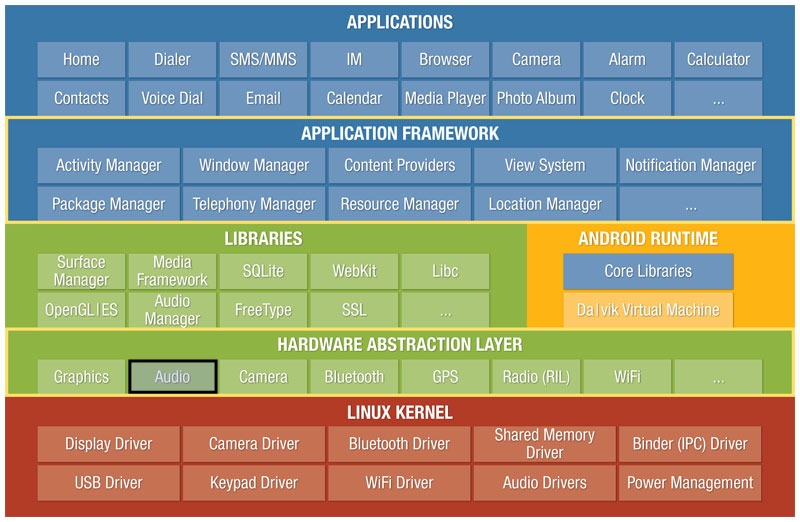
\includegraphics[width=\textwidth]{./src/img/android-archi-audio-hal.jpeg}
\end{figureGraphics}

Within the Audio feature team in Toulouse, we are mainly focused around the Audio \gls{hal}.

\subsection{Intel Audio HAL}
Intel's Audio \gls{hal} for Android platforms is based around a generic, plugin-based solution: the \gls{pfw}.
It runs in the \emph{userland}, which is easier to maintain than kernel-space code.
Since this solution is plugin-based, it is easy to extend to add more subsystems if needed.

There is an overview of the Intel Audio \gls{hal} on figure \ref{fig:hal}.
\begin{figureGraphics}{Simplified view of Intel Audio HAL}{fig:hal}
\includegraphics[height=0.5\textheight]{./src/img/hal-architecture.pdf}
\end{figureGraphics}
Two different instances of \gls{pfw} are used to communicate between the
different managers used in the \gls{hal}.

Some requirements of the Intel Audio \gls{hal}:
\begin{itemize}
    \item Since the audio system needs to be tunable by the tuning engineers, the \gls{hal} should be configurable.
        It is very painful to recompile the code at each time it is needed to adapt the value of a mixer!
    \item Since the \gls{hal} needs to \emph{abstract} the hardware variations, it should also be scalable. It should be
        easy to support new hardware.
\end{itemize}

The \gls{pfw} is a way to fill those requirements.

\section{Parameter-framework}
\label{sec:parameter-framework}
During a phone call, the smartphone isn't just transmitting the sound received from the microphone. Various algorithms are
enabled on on the signal which is transmitted and send.
Those algorithms have a lot of parameters, which can change depending on the use case: whether we are in a phone call,
or listing to some music. Furthermore, those parameters are \emph{often hardware dependent}.

To simplify the maintenance of those multiple parameters, the \gls{pfw} was born.

\subsection{Some concepts}
In this section we are going to discover the concepts which make the
\gls{pfw} such a powerful tool.

\subsubsection{Structure}
The \gls{pfw} is first of all a hierarchical tree of parameters.
On figure \ref{fig:pfwtree} we can see an example of audio tree.

\begin{figureGraphics}{Parameter framework tree example}{fig:pfwtree}
    \fbox{\begin{minipage}{6cm}
            \dirtree{%
                .1 audio.
                    .2 microphone.
                        .3 echo\_cancellation.
                            .4 enable.
                            .4 configuration.
                                .5 gain.
                                .5 coefficient.
                    .2 speaker.
                        .3 equalizer.
                            .4 enable.
                            .4 configuration.
                                .5 filter.
                                .5 coefficient.
            }
    \end{minipage}}
\end{figureGraphics}

These structures are stored in \gls{xml} files. This is great because it implies that we don't need
to recompile the \gls{pfw} when changing the structure we are describing.

In listing \ref{lst:pfwstructure}, when can see the \gls{xml} structure file
describing the tree from figure \ref{fig:pfwtree}.

\begin{code}[language=pfwXml, caption=Structure file example snippet, label=lst:pfwstructure]
<!--snippet-->
<ComponentType Name="echo_cancellation">
    <BooleanParameter Name="enable"/>
    <ParameterBlock Name="configuration">
        <IntegerParameter Name="gain" Size="8"/>
        <IntegerParameter Name="coefficient" Size="8"/>
    </ParameterBlock>
</ComponentType>
<!--snippet-->
\end{code}

\subsubsection{Settings}
The \gls{pfw} is also able to change multiple parameters without any manual action, depending on the context.
The context is defined via a set of criterion. Those criterion are variables which can take a set of defined values.
For example, a criteria called \emph{Output Device} can take several values such as \emph{Speaker} or \emph{Headset}.

Depending on the value of those criteria, the \gls{pfw} can automatically apply a set of values towards
multiple parameters.
On listing \ref{lst:pfwsettings} we can see an example of setting file.

\begin{code}[language=pfwLang, caption=Settings file example, label=lst:pfwsettings]
Domain:
    Conf: SpeakerWithEchoCancel
        OutputDevice Is Speaker
        Component: audio/microphone/
            echo_cancellation/enable = true
            configuration/gain = 2
            configuration/coefficient = 3 # arbitrary values
# -- snippet --
\end{code}

\subsubsection{Extensibility}
Since the \gls{pfw} is \emph{plugin-based}, it is easy to extend it's functionality to other usages than Audio, such
as Camera, or Bluetooth.


\subsection{Topic of my internship}
I worked within the Intel Audio development team, as an \emph{agile
software developer}. The team is customers oriented, using \gls{scrum}
methodology (see chapter \ref{chap:organisation}). My tasks
within the team were focused around enchancing and open-sourcing the \gls{pfw} on
\gls{GitHub}\footnote{\url{www.github.com/01org/parameter-framework}} to give it some
visibilty.


\section{Workflow and environment}
In this section, we will cover my daily workflow. This helps
to understand how I proceeded during my whole internship.

\begin{figureGraphics}{Developer workflow}{fig:workflow}
    \includegraphics[height=0.6\textheight]{./src/img/workflow.pdf}
\end{figureGraphics}

This workflow is the same for every developer member of the team. It is
detailed in the sub sections below.

\subsection{Development}
Since compiling the Android source tree requires a lot of computing power,
most of developers of our team are working remotely, via ssh.
The server we are connecting to is far more powerful than the desktops we use.
With it 32 cores and it's 2 TeraBytes of SSD, compilation time was far less time-consuming
than compiling locally!

I also worked on that server. This constraints to use command line programs only.
During my internship, I sharpened my skills in \gls{vim} and discovered \gls{tmux}.
On the figure \ref{fig:setup} below, there is a screenshot of my development setup at Intel.

\begin{figureGraphics}{Development setup with vim and tmux}{fig:setup}
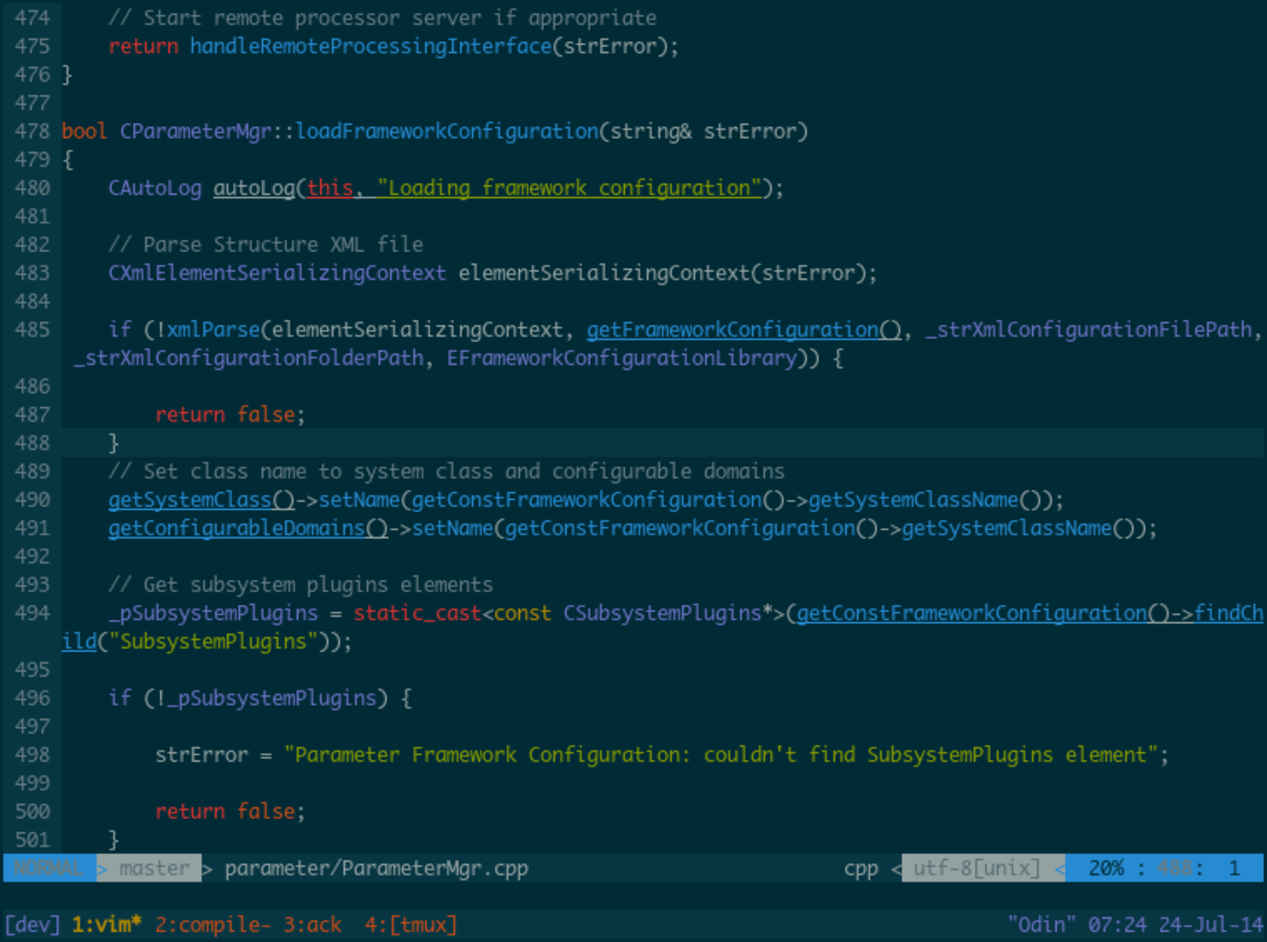
\includegraphics[width=\textwidth]{./src/img/setup.pdf}
\end{figureGraphics}

When the code is ready, I pushed it via \gls{git} on \gls{gerrit} to be reviewed.

\subsection{Code quality}
Code quality matters. Clean code eases maintenance and is less error-prone.
Those facts are driving the team that I integrated at Intel. Naturally, all the
patches I have delivered during my internship have been reviewed and meet the
expected quality.

I have done some code review myself during this internship. It helps a lot to
understand how other people work. Viewing other peoples code also makes me come
up with new ideas to improve my own work.

\subsection{Submission to integration team}
After the code is ready and validated by the development team, it is submitted towards the integration team.
They are responsible for testing complicated uses cases and validating the work the developers did.


%
% auth: Mattijs Korpershoek
% mail: <mattijs.korpershoek@gmail.com>
%
\section{Methodology}

\currentSectionToc

\subsection{Environment}
\begin{frame}
    \frametitle{Technical environment}
    \begin{minipage}{0.49\textwidth}
    \begin{itemize}
        \item Vim, Tmux, Ssh
        \item C++, Python, Bash, XML
        \item Git, Gerrit, GitHub
        \item Bugzilla
        \item Rational Team Concert
    \end{itemize}
    \end{minipage}
    \begin{minipage}{0.49\textwidth}
        \flushright
        
\includegraphics[height=1.5cm]{./img/vimLogo.png} \hspace{0.2cm}
        
\includegraphics[height=1.5cm]{./img/pythonLogo.png} \hspace{0.2cm}
        
\includegraphics[height=1.5cm]{./img/githubLogo.png} \\
        
\includegraphics[height=1.5cm]{./img/bzLogo.png} \hspace{0.2cm}
        
\includegraphics[height=1.5cm]{./img/rtcLogo.jpg}
    \end{minipage}
\end{frame}

\subsection{Agile software development}
\begin{FrameWithSubSection}
    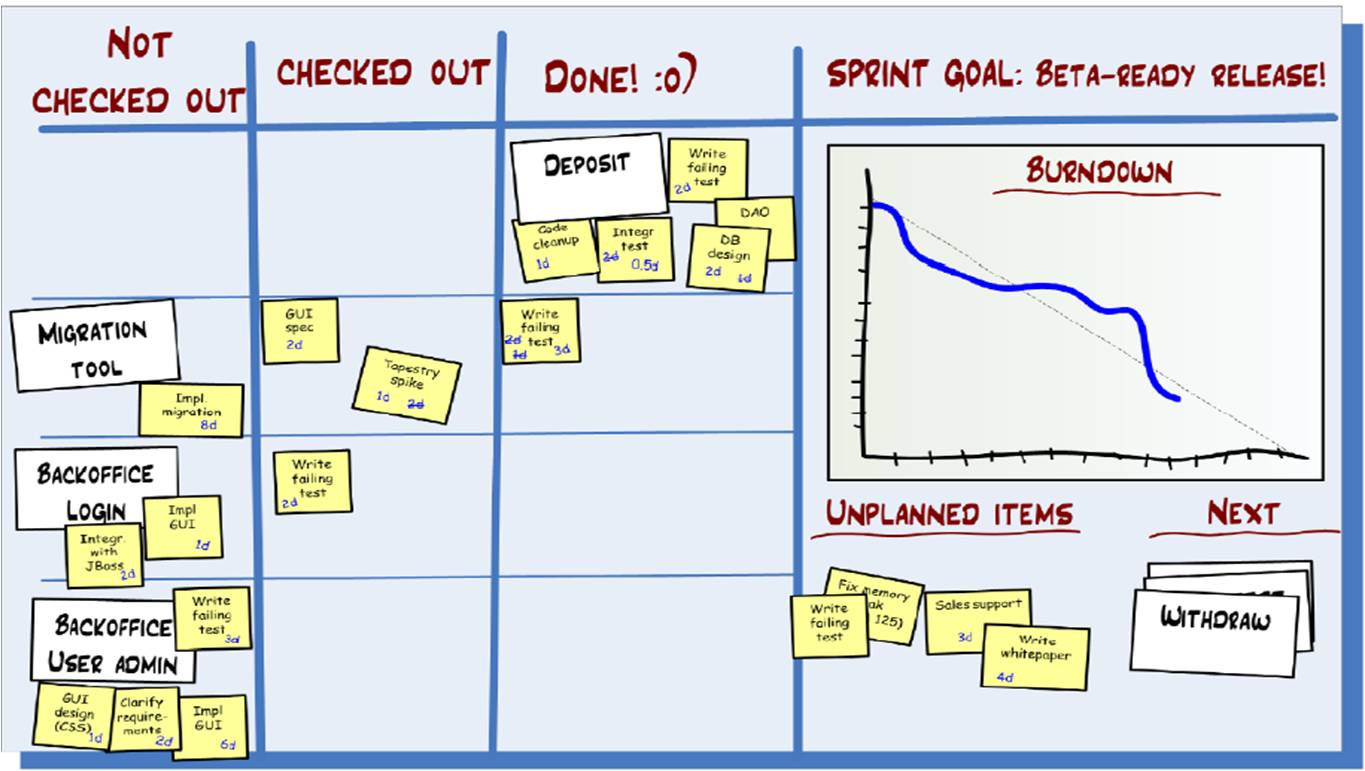
\includegraphics[width=\textwidth]{../../report/src/img/taskboard.jpg}
\end{FrameWithSubSection}

\begin{FrameWithSubSection}
    \frametitle{Agile contributions}
    \begin{minipage}{0.49\textwidth}
        \begin{itemize}
            \item Time management (\emph{Pomodoro technique}, \emph{croissant points})
            \item Pair programming
            \item Human focused retrospectives (\emph{Mad sad glad})
        \end{itemize}
    \end{minipage}
    \begin{minipage}{0.40\textwidth}
        \flushright
        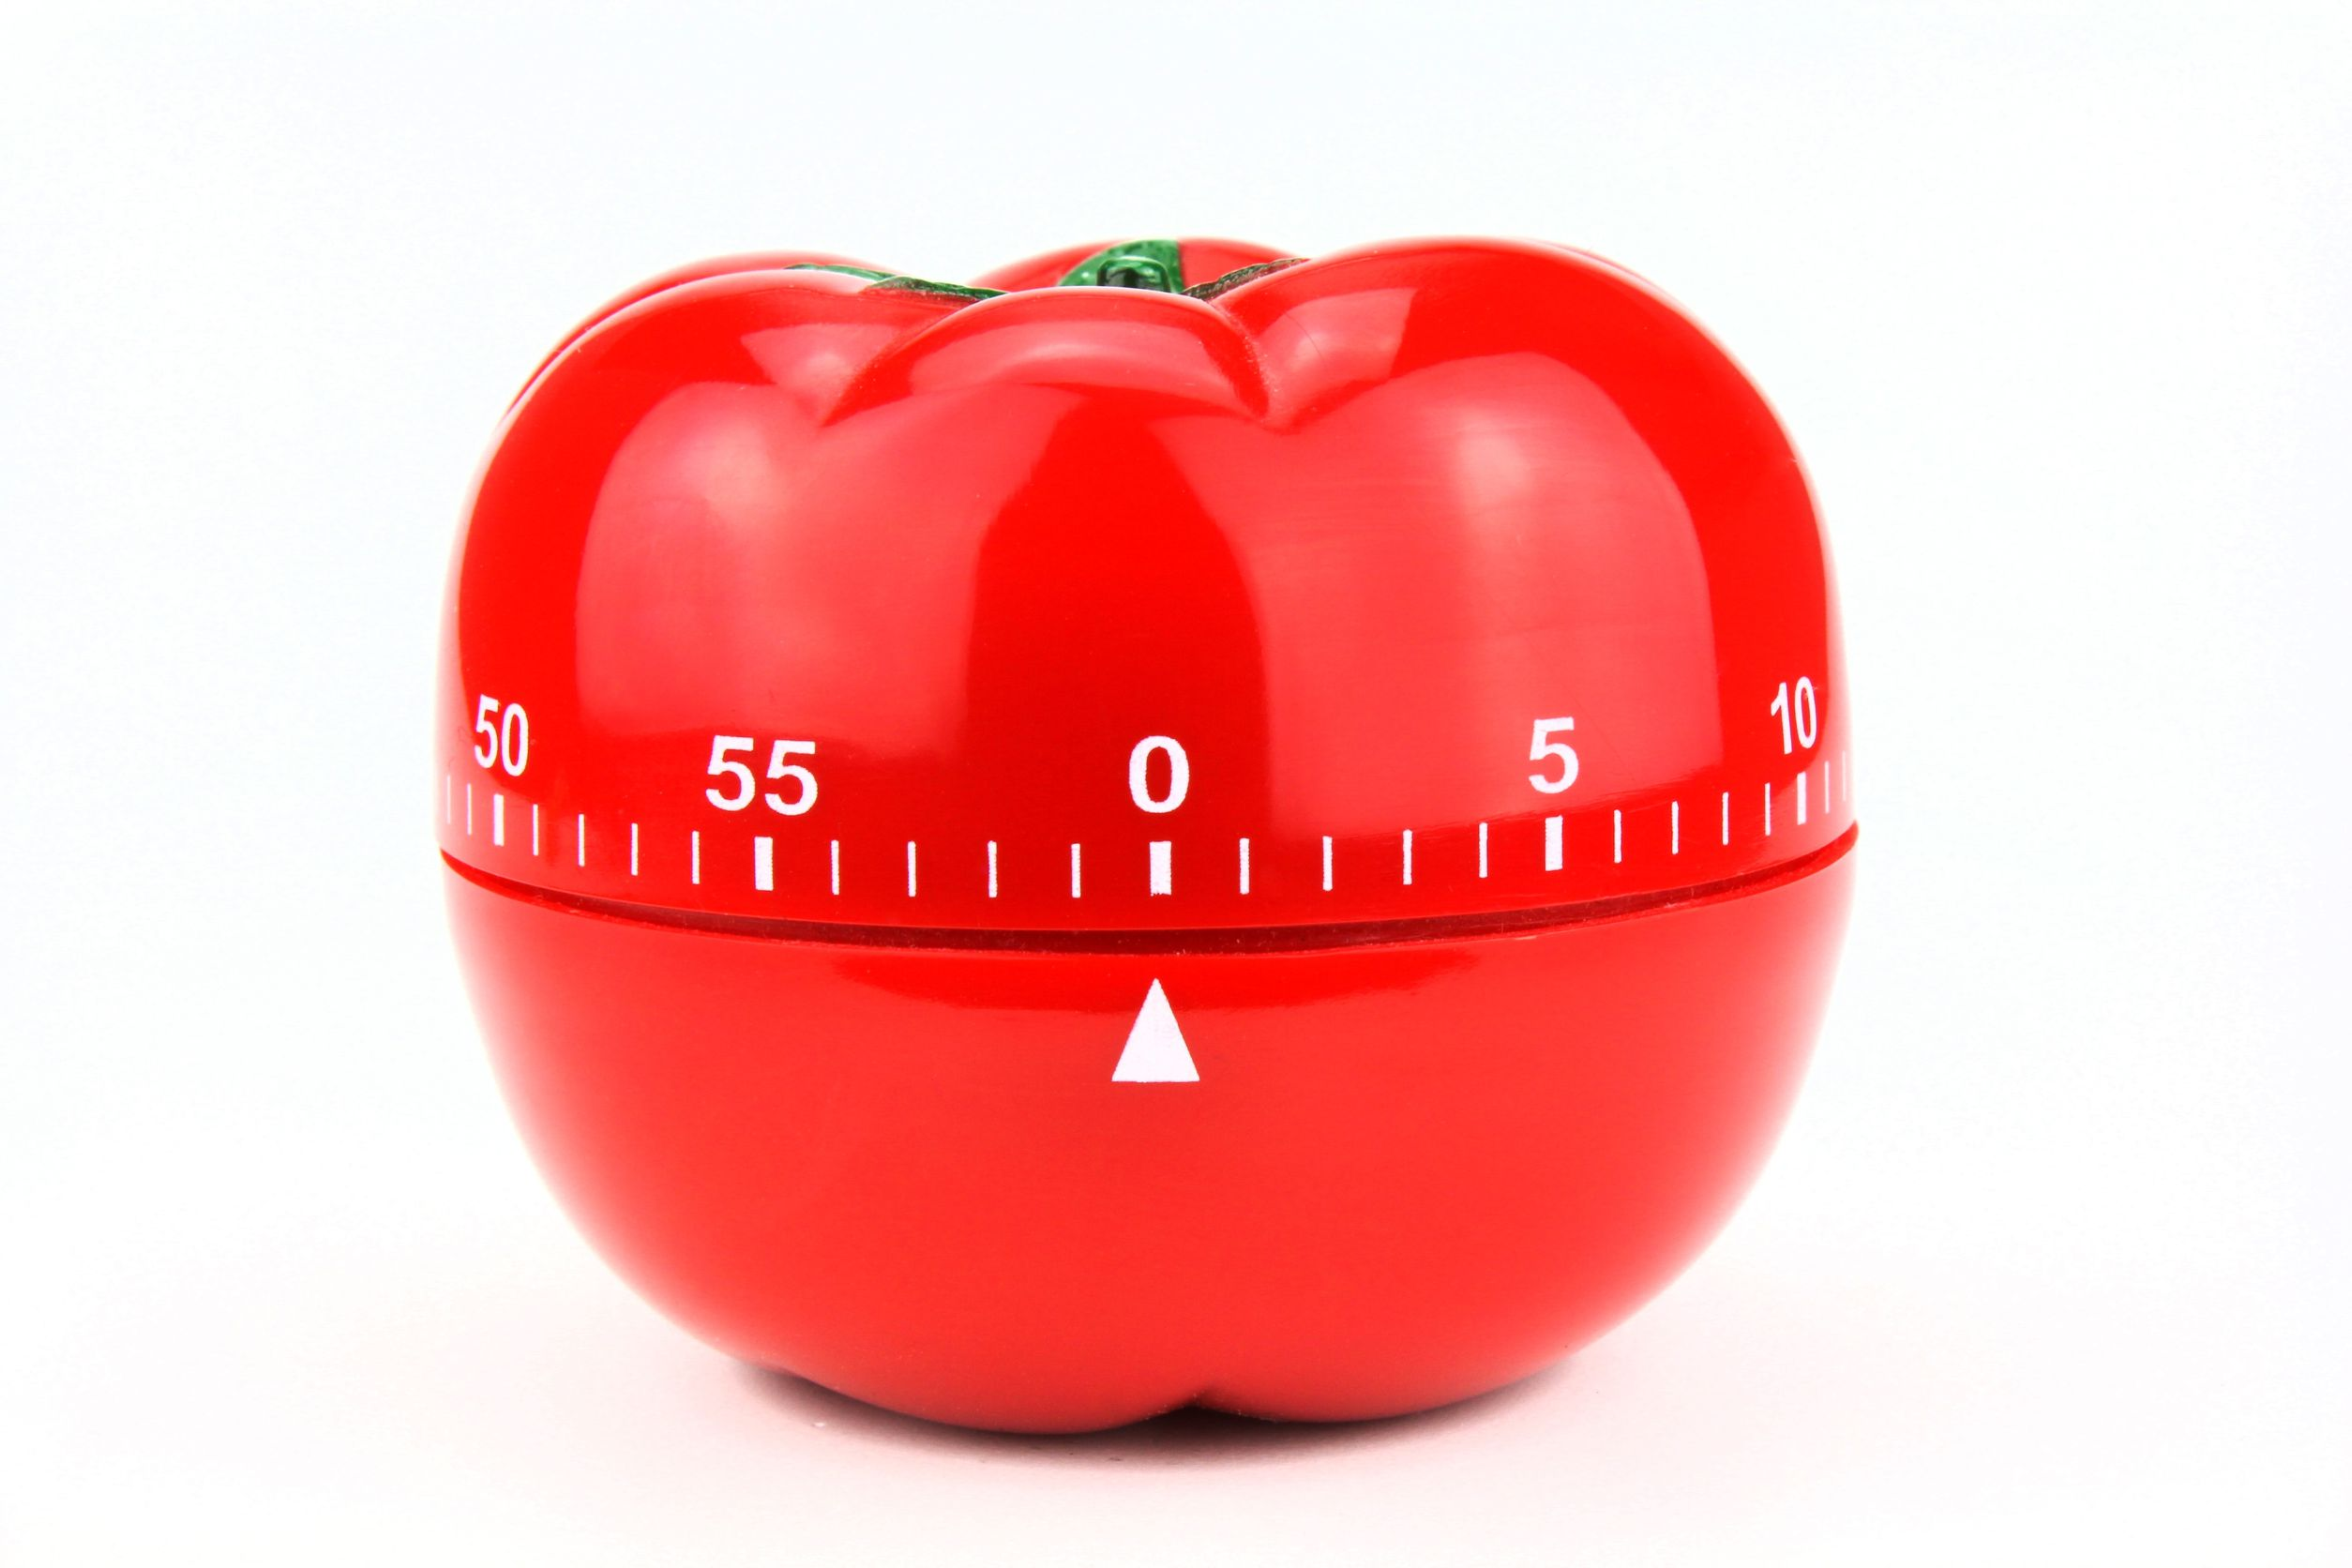
\includegraphics[width=0.40\textwidth]{./img/pomodoro.jpg} \hspace{0.2cm}
        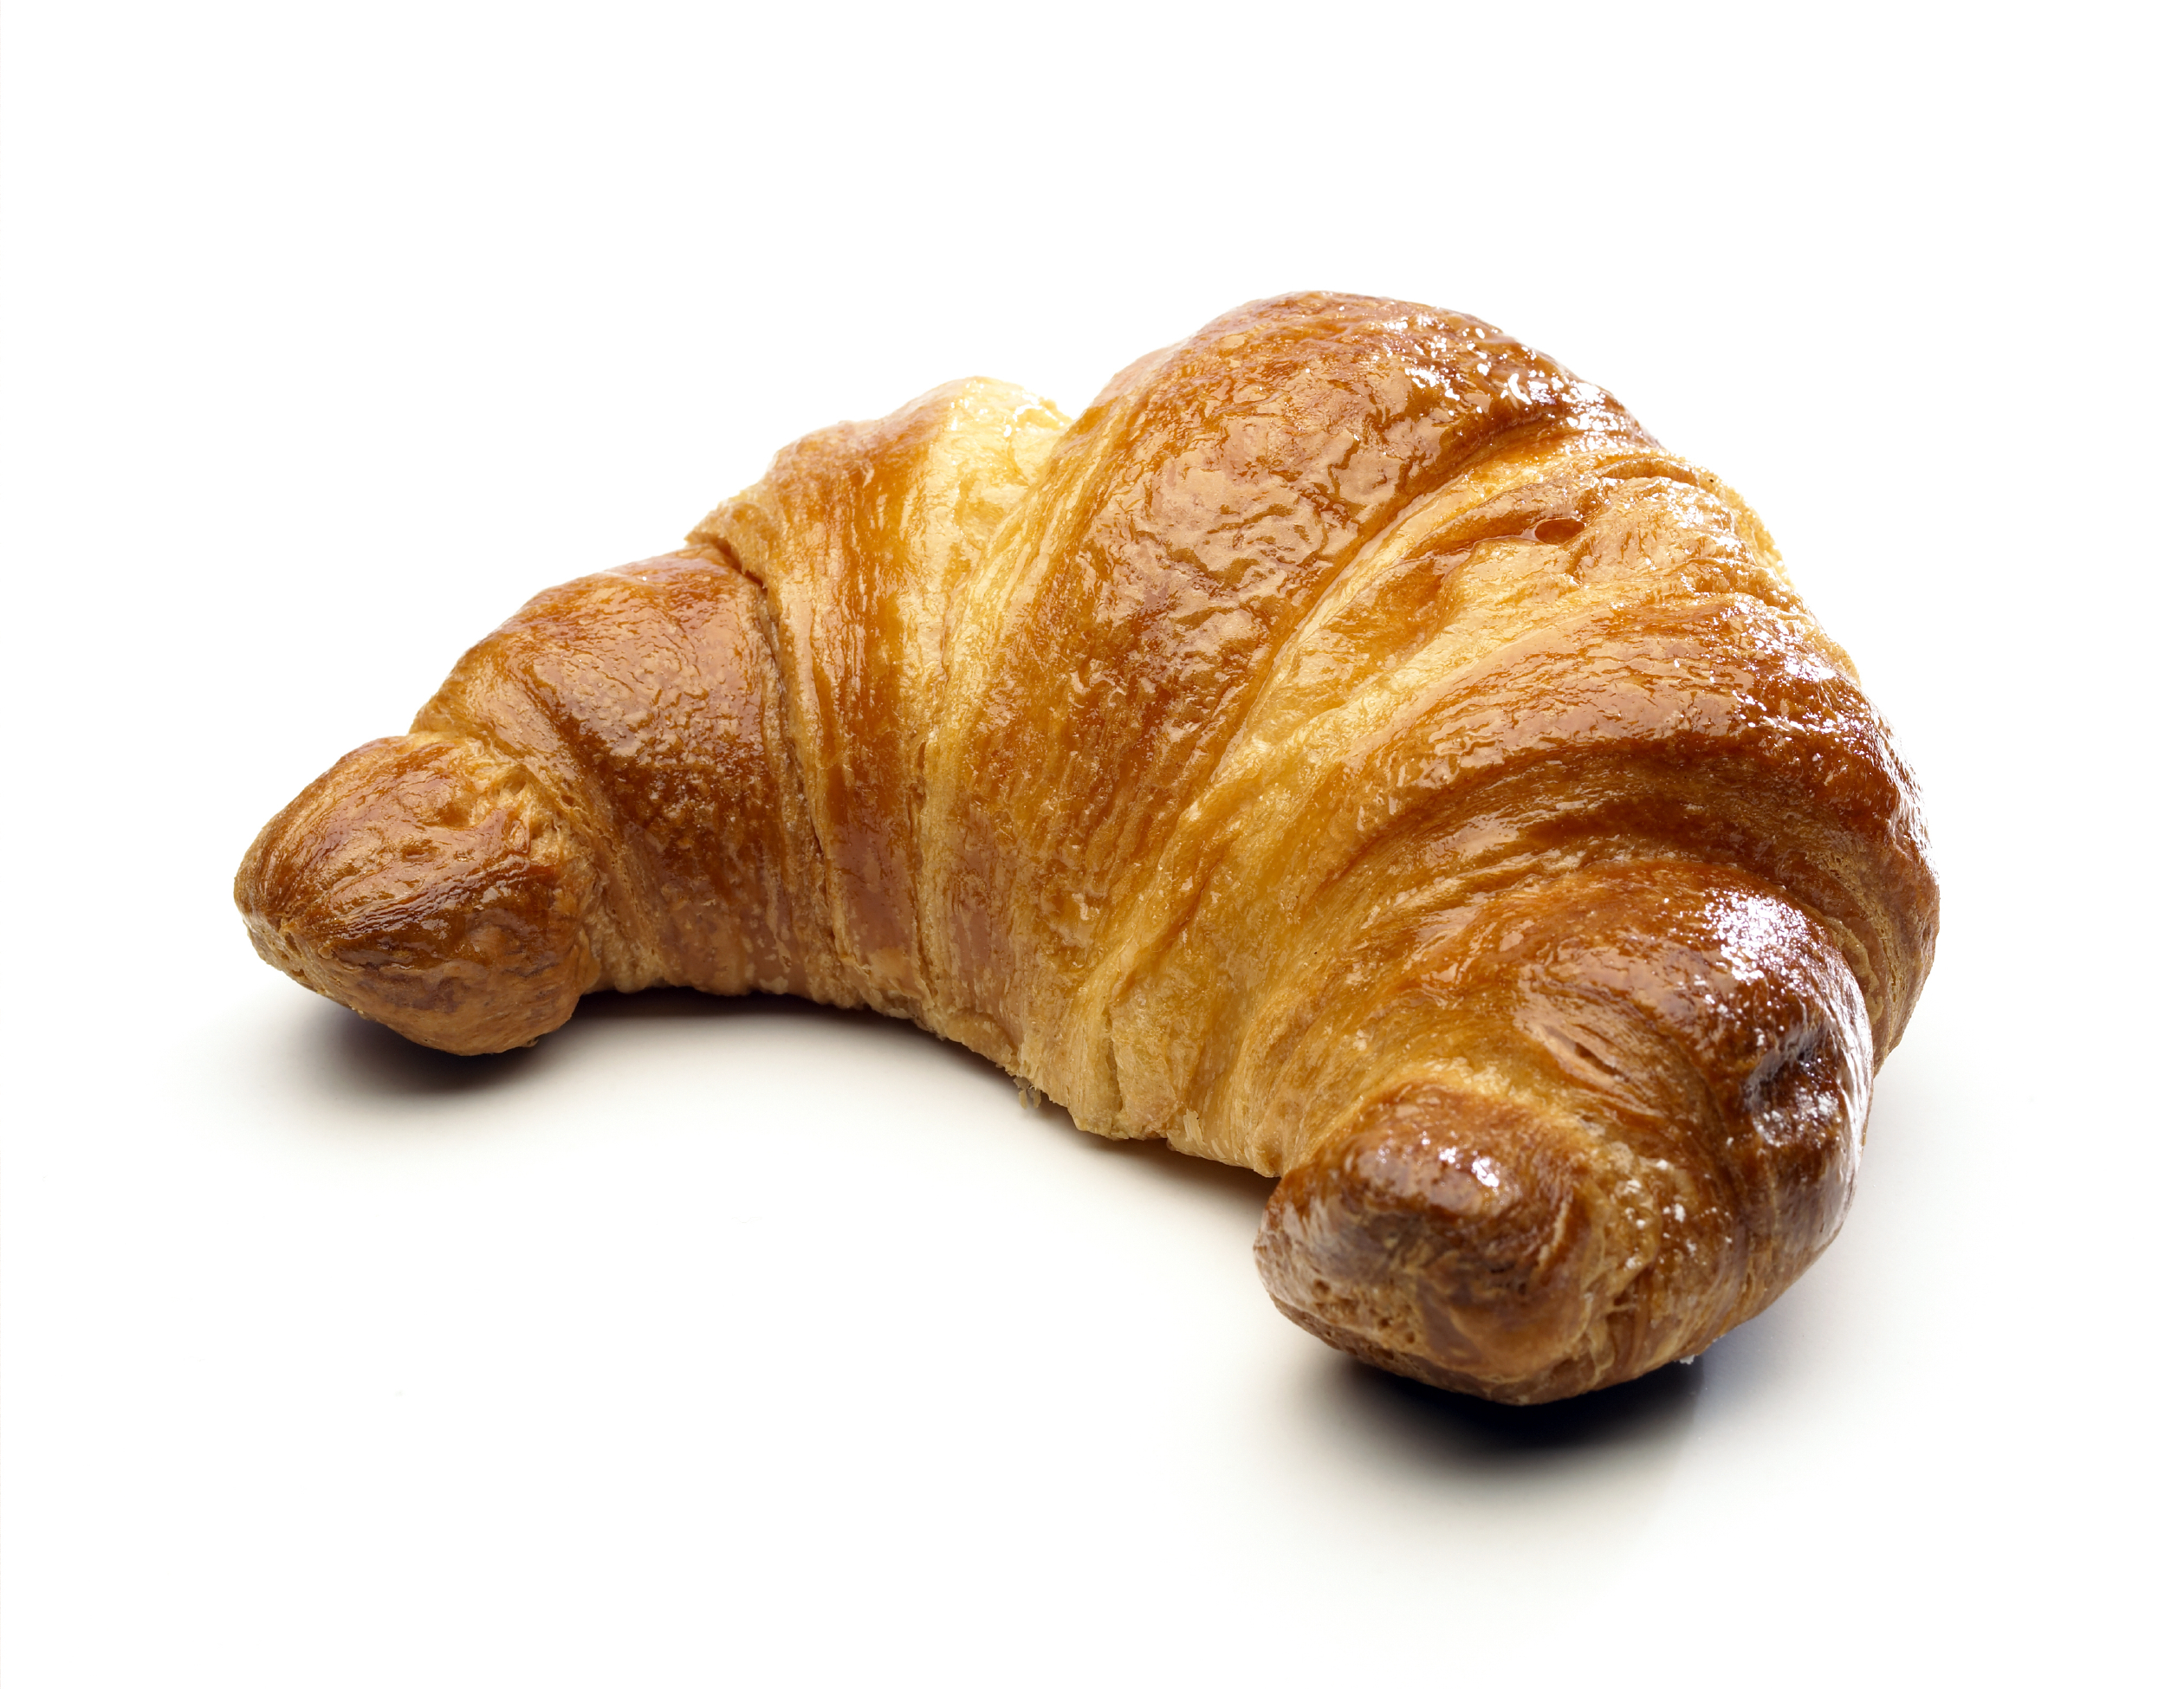
\includegraphics[width=0.40\textwidth]{./img/croissant.jpg} \\
        
\includegraphics[width=\textwidth]{../../report/src/img/mgs.png}
    \end{minipage}
\end{FrameWithSubSection}


\subsection{Gantt chart}
\begin{FrameWithSubSection}
    \hspace*{-0.8cm}
\begin{ganttchart}[
        x unit=0.35cm,
        y unit title=.4cm,
        y unit chart=.4cm,
        hgrid=true,
        vgrid={*1{red, dotted}},
        canvas/.style={fill=base2},
        bar/.style={fill=orange},
        title/.style={fill=base2},
        group/.style={fill=blue, shape=ganttgroup},
        bar height = 0.4,
        bar label font = {\scriptsize},
        title label font = {\color{blue}},
    ]{1}{24}
    \gantttitlelist[title label font={\tiny}]{1, ..., 24}{1} \\
    \ganttbar{Arrival, installation}{1}{1} \\
    \ganttgroup{\color{blue}Client deliverables}{4}{20} \\
    \ganttbar{Improving build process}{4}{11} \\
    \ganttbar{Multi-variant support}{5}{6} \\
    \ganttbar{Fixed point enhancements}{9}{11}\\
    \ganttbar{Multi modem support}{17}{20}\\
    \ganttgroup{\color{blue}Open-sourcing}{1}{20} \\
    \ganttbar{Newcomer documentation}{1}{4}\\
    \ganttbar{Intellectual property}{12}{13}\\
    \ganttbar{Alsa plugin refactor}{12}{14}\\
    \ganttbar{Filesystem plugin update}{14}{15}\\
    \ganttbar{Core update}{15}{18}\\
    \ganttbar{Alsa plugin update}{17}{20}\\
    \ganttgroup{\color{blue}University}{21}{24} \\
    \ganttbar{Internship report}{21}{24} \\
    \ganttbar{Slides internship}{23}{24}
\end{ganttchart}
\end{FrameWithSubSection}


%
% auth: Mattijs Korpershoek
% mail: <mattijs.korpershoek@gmail.com>
%

% {{{1 intro
\section{Technical contributions}
\subsection{Directions}
\begin{FrameWithSubSection}
    \begin{itemize}
        \item Customer features
        \item Open-sourcing a core component
    \end{itemize}
\end{FrameWithSubSection}


% {{{1 Customer features
\subsection{Features for customers}
\begin{FrameWithSubSection}
    \begin{itemize}
        \item More than \emph{80} patches delivered
        \item Code integrated into Intel's code base
        \item Software quality compliant
    \end{itemize}
\end{FrameWithSubSection}

% {{{2 xml validation
\subsubsection{Xml Validation at build time}
\begin{frame}
    \frametitle{XML Validation at build time}
    \begin{minipage}{0.4\textwidth}
        \begin{itemize}
            \item More than 40 000 lines of XML
            \item More than 500 errors within those files
            \item Automatic validation with XSD at build time
            \item Prevents from submitting erroneous data
        \end{itemize}
    \end{minipage}
    \begin{minipage}{0.5\textwidth}
        \flushright
        \includegraphics[height=0.85\textheight]{../../report/src/img/build-generation-after.pdf}
    \end{minipage}
\end{frame}

% {{{2 fixed point
\subsubsection{Fixed point parameter improvements}
\begin{frame}
    \frametitle{Fixed point parameter improvements}
    \begin{minipage}{0.5\textwidth}
        \begin{block}{Fixed point numbers}
            \begin{itemize}
                \item $Qn.m$ notation
                    \begin{itemize}
                        \item $n$ : fractional part
                        \item $m$ : integral part
                    \end{itemize}
                \item Rounding issues with conversion to floating point
                \item \lstinline{std::setPrecision()}
            \end{itemize}
        \end{block}
    \end{minipage}
    \begin{minipage}{0.4\textwidth}
        \flushright
        \begin{block}{Solution}
            \begin{itemize}
                \item Simple and elegant solution
                \item Behavior test suite
                \item Used in multiple Intel products
            \end{itemize}
        \end{block}
    \end{minipage}
    \begin{minipage}{\textwidth}
        \flushright
        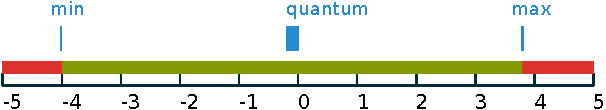
\includegraphics[width=\textwidth]{../../report/src/img/fixedPoint.pdf}
    \end{minipage}
\end{frame}

% {{{2 multimodem

\subsubsection{Multi modem support}
\begin{frame}
    \frametitle{Modem instance awareness}
    \begin{itemize}
        \item Voice processing algorithms
        \item Multiple modems for several phone carriers
        \item Big team effort of more than 200 patches
        \item Parameter-framework modem plugin
    \end{itemize}
\end{frame}

% {{{1 Opensourcing
\subsection{Open-sourcing the Parameter-framework}
\subsubsection{Context}
\begin{FrameWithSubSection}
    \begin{block}{Why open-sourcing this component?}
        \begin{itemize}
            \item Core component of Intel audio HAL
            \item Potential to become middleware standard
            \item Visibility
        \end{itemize}
    \end{block}
\end{FrameWithSubSection}

\subsubsection{Documentation}
\begin{frame}
    \frametitle{Newcomer documentation}
    \centering
    \begin{block}{Is the component ready for open-sourcing?}
        \begin{itemize}
            \item Code review and study
            \item Documentation for external contributors
            \item More than 450 lines of documentation
        \end{itemize}
    \end{block}
\end{frame}

\begin{frame}
    \frametitle{Newcomer documentation illustration}
    \centering
    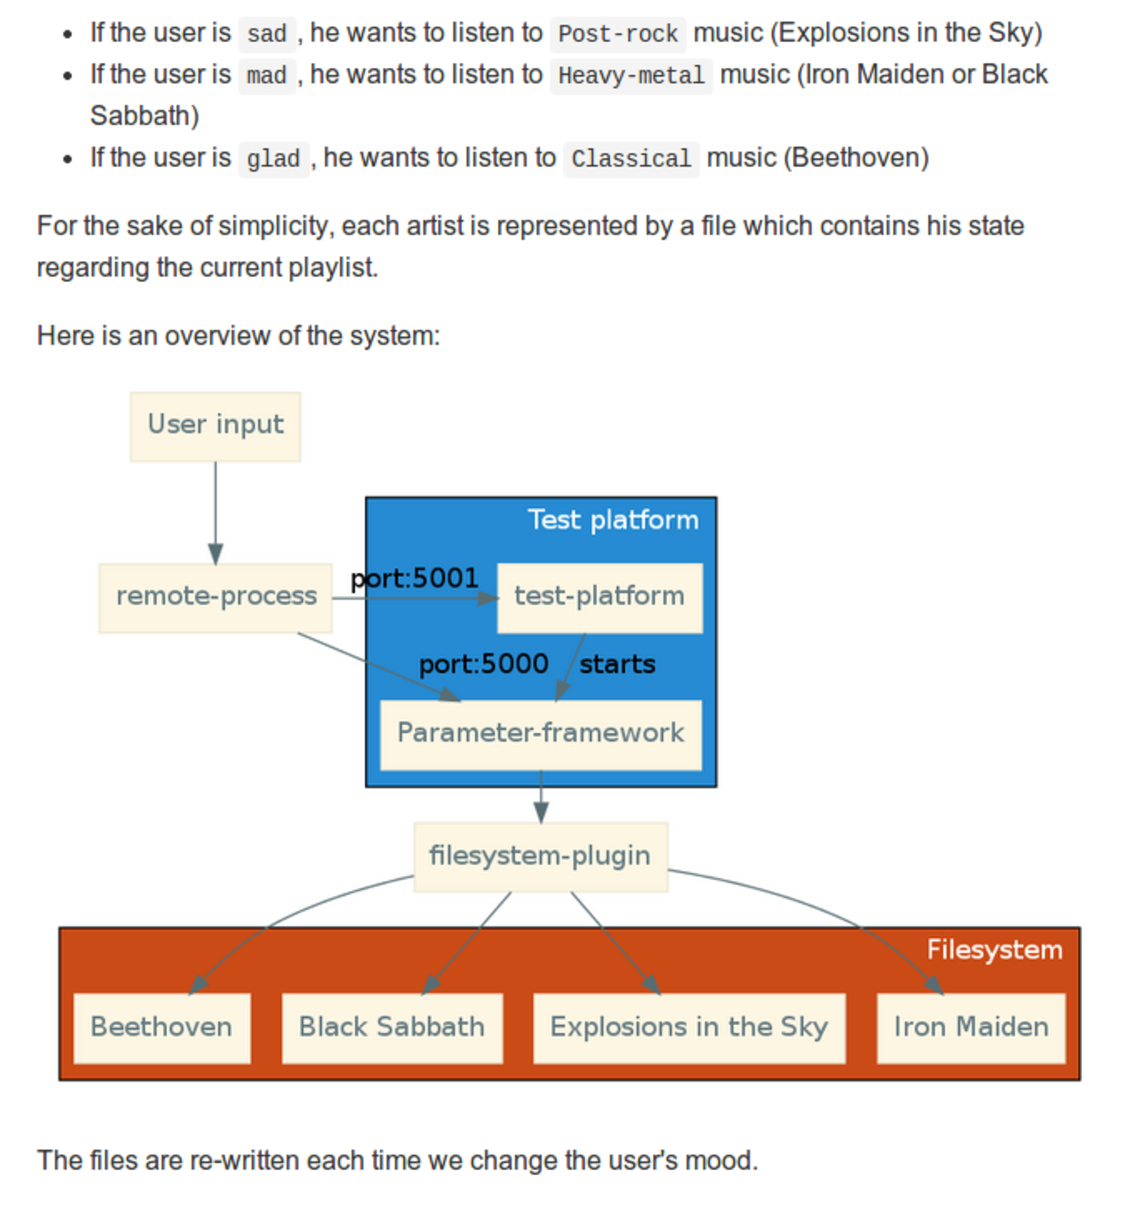
\includegraphics[height=0.85\textheight]{../../report/src/img/tutos.pdf}
\end{frame}

\subsubsection{Branch sync process}
\begin{frame}
    \frametitle{Branch sync process}
    \begin{block}{How to open-source the component?}
        \begin{itemize}
            \item Ensure external contributions are of quality
            \item Avoid maintenance of 2 divergent code bases
            \item Ensure no confidential information is exposed
        \end{itemize}
    \end{block}
\end{frame}

\begin{frame}
    \frametitle{Branch sync process}
    \centering
    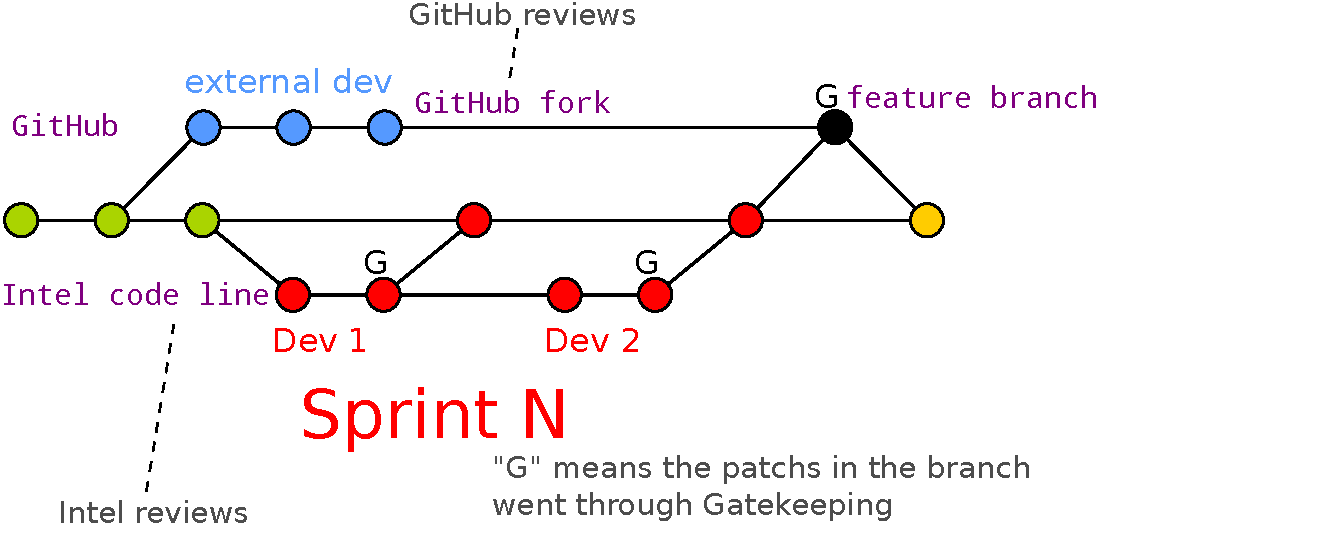
\includegraphics[width=\textwidth]{../../report/src/img/branches-process.pdf}
\end{frame}

\subsubsection{Open-sources projects}
\begin{frame}
    \frametitle{Projects which are open-source}
    \begin{block}{01org}
        \begin{itemize}
            \item \href{https://01.org/}{Intel Open Source Technology Center}
            \item \href{https://github.com/orgs/01org/teams/01-org-parameter-framework-owners}{GitHub organisation}
        \end{itemize}
   \end{block}
    \begin{block}{Projects on GitHub}
        \begin{itemize}
            \item Parameter-framework \href{https://github.com/01org/parameter-framework}{core}
            \item Parameter-framework \href{https://github.com/01org/parameter-framework-plugins-alsa}{ALSA plugin}
            \item Parameter-framework \href{https://github.com/01org/parameter-framework-plugins-filesystem}{filesystem plugin}
            \item Parameter-framework \href{https://github.com/01org/parameter-framework/wiki}{wiki}
            \item Parameter-framework \href{https://github.com/01org/parameter-framework-samples}{sample files}
        \end{itemize}
    \end{block}
\end{frame}

\begin{frame}
    \frametitle{GitHub top contributors}
    \centering
    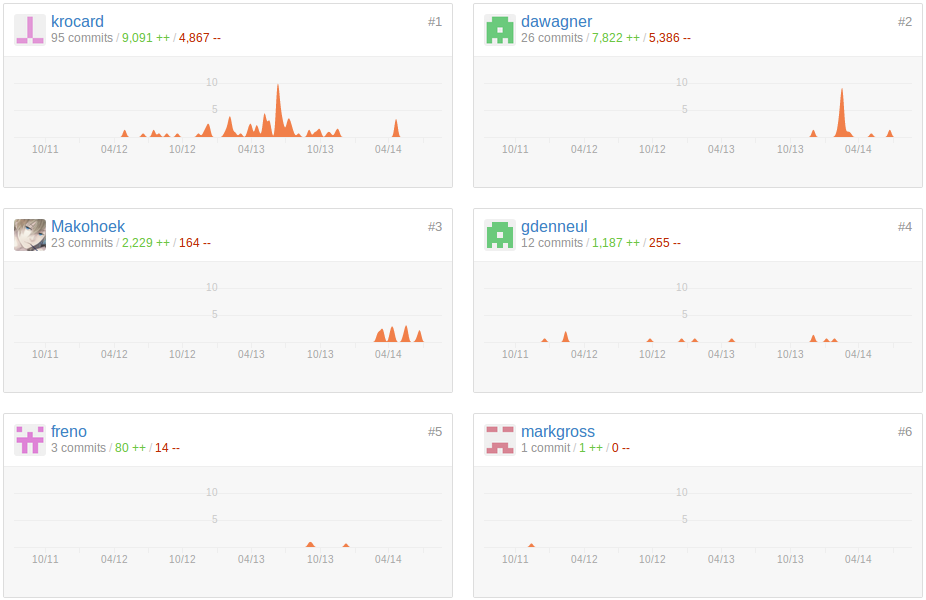
\includegraphics[width=\textwidth]{../../report/src/img/statsGitHub.png}
\end{frame}

\chapter{Conclusion}

\section{Outcomes}

\subsection{Added value of my work}
\subsubsection{Scrum improvements}
During my internship, I came up with some fresh ideas about how to enhance the \gls{scrum} process within the team.
Several improvements have been made, such as better retrospectives and better demo preparation.
Building team spirit is essential in an effective \gls{scrum} team, something I managed to catalyze within the team.
This has convinced me more than all that \gls{scrum} is simple to learn, but very hard to master.
It is more than just a way to organize work. It is a different mindset to have. And it is a lot of fun!

\subsubsection{Technical side}
All the contributions listed in chapter \ref{chap:contributions} are integrated into Intel's codebase.
This code is used on a daily basis by thousands of developers. There will be products shipped running the
code I developed within the team.
Regarding the open-source documentation, it is available on \gls{GitHub}.

\subsection{Areas of improvement}
Even if I did a lot of different things related to the \gls{pfw}, there are still many things to do.
In order to stimulate the adoption of the \gls{pfw}, it would be great to
port and open-source the Intel audio \gls{hal} to well-known development boards for example a
Pandaboard, a Raspberry Pi or a Beaglebone.


\section{Personal outcome}

For my internship, I was looking for a good technical challenge. I found the right place
at Intel's audio team.
This is one of the most complex (and also one of the most
interesting) project I have ever worked on!

\subsection{Consistency with university classes}
Even if I had a solid technical background thanks to the courses of my
\gls{camsi} Master, there were some skills which I lacked.
I missed especially some skills about advanced \gls{cpp} and some "good software practices".

In contrary, there were also a lot of things which helped me a lot during
my internship.  During the \gls{camsi} Master, we made a lot of stimulating
projects. From creating a simple thermal driver to building our own quadcopter
and make it fly, we really covered various topics! This \emph{all-around} set of
skills helped me to quickly adapt to the requirements at Intel.

\subsection{Career perspectives}
During my internship I was also searching for a job in September. Celad offered me a position to work
as contractor at Intel in the same team I worked with for six months.
Since I learned a \emph{lot} during my internship, I can't wait to continue learning more and follow my career
as an agile software developer!

\section{Conclusion}
The satisfaction of learning new things is a daily feeling I have at
Intel. Android is huge. The knowledge within the team is huge as well. I can't
wait to contribute more within Intel's audio team!


\end{document}
